\documentclass[12pt]{article}

\usepackage[utf8]{inputenc}
\usepackage[italian]{babel}
\usepackage{enumitem}
\usepackage{graphicx}
\usepackage{listings}
\usepackage{xcolor}
\usepackage{float}

\usepackage[backend=bibtex,sorting=none]{biblatex}
\addbibresource{references.bib}

\definecolor{codegreen}{rgb}{0,0.6,0}
\definecolor{codegray}{rgb}{0.5,0.5,0.5}
\definecolor{codepurple}{rgb}{0.58,0,0.82}
\definecolor{backcolour}{rgb}{0.95,0.95,0.92}
\lstdefinestyle{mystyle}{
    backgroundcolor=\color{backcolour},   
    commentstyle=\color{codegreen},
    keywordstyle=\color{magenta},
    numberstyle=\tiny\color{codegray},
    stringstyle=\color{codepurple},
    basicstyle=\ttfamily\footnotesize,
    breakatwhitespace=false,         
    breaklines=true,                 
    captionpos=b,                    
    keepspaces=true,                 
    numbers=left,                    
    numbersep=5pt,                  
    showspaces=false,                
    showstringspaces=false,
    showtabs=false,                  
    tabsize=2
}

\lstset{style=mystyle}

\title{Analisi di Yelp Open Dataset}
\author{
        Lorenzo Vainigli\\
        \textit{\small Corso di Intelligenza Artificiale a.a. 2019/20}\\
        \textit{\small Laurea Magistrale in Informatica}\\
        \textit{\small Università di Bologna}
}
\date{}

\begin{document}
\maketitle
\tableofcontents

\section{Introduzione}
I file di questo progetto sono disponibili nel repository dell'autore su GitHub \cite{repo}. 

\section{Dati}
\textit{Yelp Open Dataset} \cite{yelp} è una base di dati che raccoglie informazioni su esercizi commerciali di varie categorie. I dati sono utilizzabili per uso personale, educativo o accademico, sono disponibili in formato JSON e sono divisi in alcuni file:
\begin{itemize}
\item \textit{business.json} (153 MB): contiene le informazioni relative agli esercizi commerciali tra cui ubicazione e categoria.
\item \textit{review.json} (6,33 GB): contiene i testi delle recensioni includendo l'identificativo dell'utente che ha scritto la recensione e l'esercizio commerciale oggetto della recensione.
\item \textit{user.json} (3,27 GB): contiene i dati associati ai singoli utenti, inclusi gli identificativi degli amici.
\item \textit{tip.json} (263 MB): contiene dei suggerimenti che gli utenti scrivono a proposito degli esercizi commerciali. Possono essere visti come delle brevissime recensioni.
\end{itemize}
Il database contiene anche i file \textit{checkin.json} e \textit{photos.json}, ma non sono stati presi in considerazione per lo sviluppo di questo progetto.

\section{Obiettivi}
Lo scopo del progetto prevede l'analisi dei dati al fine di studiare la loro struttura e il loro contenuto, al fine di estrapolare osservazioni interessanti su di essi. Non si tratta solo di aggregare record o trovare valori minimi, massimi o medi, ma di applicare anche tecniche di NLP e machine learning. In partcolare, le finalità del progetto richiedono:
\begin{enumerate}[label=T\arabic*)]
\item il riconoscimento automatico di una review positiva o negativa;
\item il raggruppamento degli utenti in base alle loro preferenze o compor-
tamento sulla piattaforma;
\item il raggruppamento automatico dei locali in base a criteri di similitudine data una certa località.
\end{enumerate}
A queste, ne sono state aggiunte altre:
\begin{enumerate}[label=T\arabic*)]
\setcounter{enumi}{3}
\item analisi dei singoli file JSON;
\item classificazione dei locali migliori e peggiori per ogni categoria;
\item locali aperti nelle vicinanze dell'utente;
\item utenti con le recensioni più affidabili (comparando il loro voto alla media dei voti di un determinato locale);
\item migliori recensioni e suggerimenti (tips) per un locale.
\end{enumerate}

\section{Strumenti}
Per conseguire gli obiettivi sopra citati i dati sono stati elaborati in Python con l'utilizzo di Jupyter Notebook \cite{jupyter}.

\section{Sviluppo}
Per ogni obiettivo (o target) T* è stato creato un notebook presente nella cartella \texttt{notebooks}:
\begin{enumerate}[label=T\arabic*)]
\item \texttt{reviews\_classification.ipynb};
\item \texttt{users\_grouping.ipynb};
\item \texttt{businesses\_grouping.ipynb};
\item \texttt{business.ipynb}, \texttt{review.ipynb}, \texttt{tip.ipynb}, \texttt{user.ipynb};
\item \texttt{best\_and\_worst\_businesses.ipynb};
\item \texttt{closest\_opened\_businesses.ipynb};
\item \texttt{best\_reviewers.ipynb};
\item \texttt{best\_business\_tips.ipynb}.
\end{enumerate}
\subsection{Caricamento dei dati}
Per motivi di performance non è stato possibile analizzare tutto il contenuto dei file \textit{review.json} e \textit{user.json}, poiché troppo grandi.

\section{Risultati}

\subsection{Esercizi commerciali}
Il file \textit{business.json} contiene 209.393 record, ognuno composto da 14 campi: \textit{address}, \textit{attributes}, \textit{business\_id},	\textit{categories}, \textit{city}, \textit{hours}, \textit{is\_open},	\textit{latitude} \textit{longitude}, \textit{name}, \textit{postal\_code}, \textit{review\_count}, \textit{stars} e \textit{state}.

\subsubsection{Migliori e peggiori}
Per questa classificazione sono stete prese in considerazione il numero di stelle assegnate a ogni esercizio commerciale e il numero di recensioni ricevuto. Si presume che, a partità di stelle, più il numero di recensioni è alto, più questo valore sia affidabile. \newline
Sono state analizzate quattro delle categorie più diffuse: \textit{Restaurants}, \textit{Shopping}, \textit{Health \& Medical} and \textit{Automotive}.\newline
\textbf{Little Miss BBQ} (Phoenix, AZ), \textbf{Brew Tea Bar} (Las Vegas, NV) e \textbf{Cocina Madrigal} (Phoenix, AZ) sono i migliori ristoranti secondo la media delle stelle e il numero di recensioni ricevute, mentre \textbf{McDonald's} (Las Vegas, NV), \textbf{KFC} (Avondale, AZ) e \textbf{McDonald's} (Fort Mill, SC) sono i peggiori.\newline
Tra i negozi catalogati come \textit{Shopping}, i migliori sono \textbf{Eco-Tint} (Las Vegas, NV), \textbf{Studio 21 Tattoo Gallery} (Las Vegas, NV) e \textbf{FINO for MEN} (Las Vegas, NV). I peggiori sono \textbf{DIRECTV} (Phoenix, AZ), \textbf{Bank of America Store and Heritage Center} (Charlotte, NC) e \textbf{Teleflora Fresh Flowers} (Las Vegas, NV). \newline
\textbf{Bangkok Thai Spa Massage} (Las Vegas, NV), \textbf{Simply Skin Las Vegas} (Las Vegas, NV) e \textbf{Richards Cosmetic Surgery, Med Spa \& Laser Center} (Las Vegas, NV) sono i luoghi migliori per la categoria \textit{Health \& Medical}. Sempre per quanto riguarda questa categoria, i luoghi peggiori sono \textbf{SilverScript Medicare} (Phoenix, AZ), \textbf{Apria Healthcare} (Henderson, NV) e \textbf{OptumCare Primary Care - Deer Valley} (Phoenix, AZ).\newline
I migliori esercizi commerciali per \textit{Automotive} sono \textbf{Eco-Tint} (Las Vegas, NV), \textbf{Precision Window Tint} (Henderson, NV) e \textbf{DC Auto Luxury Window Tinting} (Las Vegas, NV). I peggiori sono \textbf{Phoenix Car Rental} (Phoenix, AZ), \textbf{LendingTree} (Charlotte, NC) e \textbf{Seller Networks} (Las Vegas, NV).\newline
Considerando le città, \textbf{Las Vegas} è quella dove si possono trovare gli esercizi commerciali migliori, considerando queste quattro categorie, seguita da \textbf{Phoenix}.

\subsubsection{Categorie}
Le categorie presenti sono in totale 1.207 e le più diffuse sono \textbf{Restaurants} (13,5\%), \textbf{Shopping} (10,7\%), \textbf{Home Services} (8,2\%), \textbf{Food} (7,7\%), \textbf{Health \& Medical} (6,8\%), \textbf{Beauty \& Spas} (13,5\%), \textbf{Local Services} (5,5\%), \textbf{Automotive} (4,6\%), \textbf{Nightlife} (4,4\%) e \textbf{Event Planning \& Services} (13,5\%).

\subsubsection{Ubicazione}
Le città in cui si trovano i locali sono 1.306. La maggior parte dei locali si trova a \textbf{Las Vegas} (15\%), seguita da \textbf{Toronto} (10\%), \textbf{Phoenix} (10\%), \textbf{Charlotte} (5\%) e \textbf{Scottsdale} (4\%).\newline
Se si effettua il raggruppamento per Stato, allora il 29\% si trova in \textbf{Arizona (AZ)}, il 19\% in \textbf{Nevada (NV)}, il 17\% in \textbf{Ontario (ON)}, l'8\% in \textbf{Ohio (OH)} e l'8\% in \textbf{North Carolina (NC)}. I restanti sono divisi tra altri Stati.

\subsection{Utenti}
Per questioni di performance e di limiti di memoria per l'elaborazione sono stati caricati sono i primi 100.000 record del file \textit{user.json}, che è composto dai campi \textit{average\_stars}, \textit{fans}, \textit{friends}, \textit{name}, \textit{review\_count}, \textit{useful}, \textit{user\_id}, e altri campi di minore importanza. \newline
Per gli utenti è stato ritenuto utile esaminare la distribuzione dei valori per i campi \textit{average\_stars}, \textit{fans} e \textit{review\_count},

\subsubsection{Distribuzione di \textit{average\_stars}}
Questo campo rappresenta la media delle stelle assegnate alle recensioni del singolo utente e, a differenza di tutti gli altri campi, presenta una distribuzione simile a una gaussiana.
\begin{figure}[H]
\centering
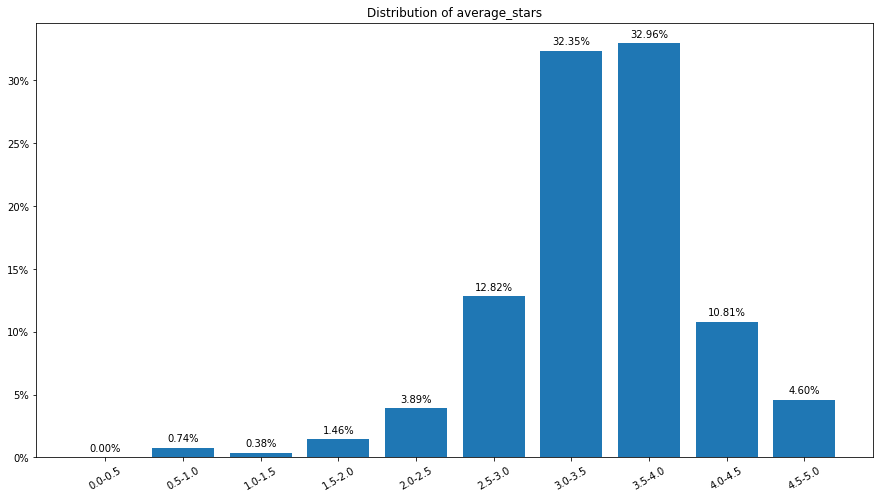
\includegraphics[width=\textwidth]{images/average_stars_distribution.png}
\caption{Distribuzione dei valori del campo \textit{average\_stars} in termini percentuali.}
\end{figure}

\subsubsection{Distribuzione di \textit{fans}}
Il 98,96\% degli utenti presenta un numero di fan tra 0 e 109 e l'81,71\% di questi ha meno di 6 fan. Questi valori portano alla conclusione che la user base di questo dataset è prevalentemente composta da utenti che interagiscono con una piccola cerchia di altri utenti.

\subsubsection{Distribuzione di \textit{review\_count}}
Questo valore dà una precisa indicazione del contributo che un utente apporta al dataset. Dall'analisi emerge che il 99,25\% degli utenti ha scritto meno di 1032 recensioni, ma è una percentuale plausibile. Molto più interessante è esaminare la segmentazione degli utenti per quanto riguarda coloro che hanno scritto meno di 100 recensioni.
\begin{figure}[H]
\centering
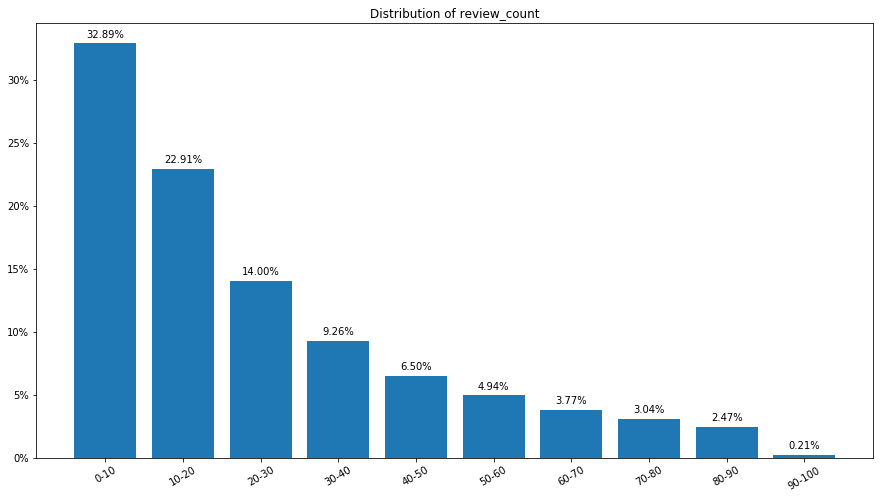
\includegraphics[width=\textwidth]{images/review_count_distribution.png}
\caption{Distribuzione dei valori del campo \textit{review\_count} per valori tra 0 e 100 in termini percentuali.}
\end{figure}

\subsection{Classificazione delle recensioni}

\subsubsection{Configurazioni della rete neurale}
\lstinputlisting[language=Python]{code_snippets/nn_config1.py}
\lstinputlisting[language=Python]{code_snippets/nn_config2.py}

\begin{figure}[H]
\centering
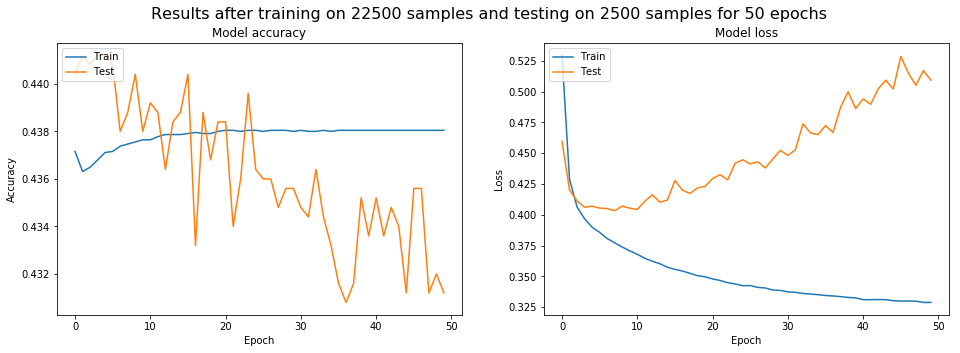
\includegraphics[width=\textwidth]{images/config1_25000samples_50epochs.png}
\caption{Risultati di \textit{accuracy} e \textit{loss} dopo un training della rete neurale in configurazione 1 con 22.500 esempi e testing con 2.500 esempi per 50 iterazioni.}
\end{figure}

\begin{figure}[H]
\centering
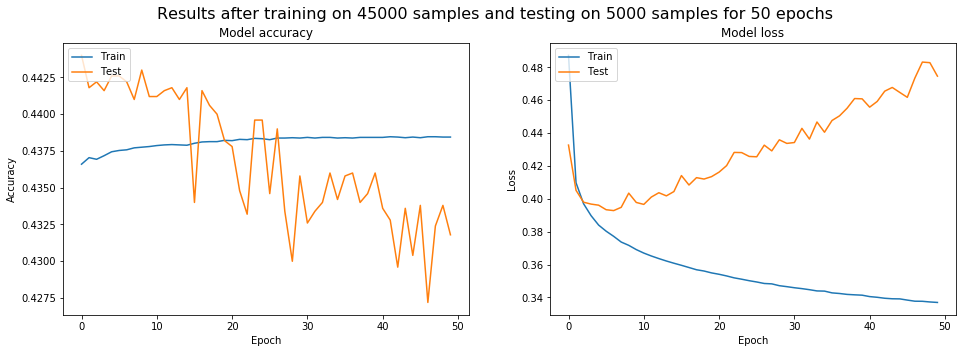
\includegraphics[width=\textwidth]{images/config1_50000samples_50epochs.png}
\caption{Risultati di \textit{accuracy} e \textit{loss} dopo un training della rete neurale in configurazione 1 con 45.000 esempi e testing con 5.000 esempi per 50 iterazioni.}
\end{figure}

\begin{figure}[H]
\centering
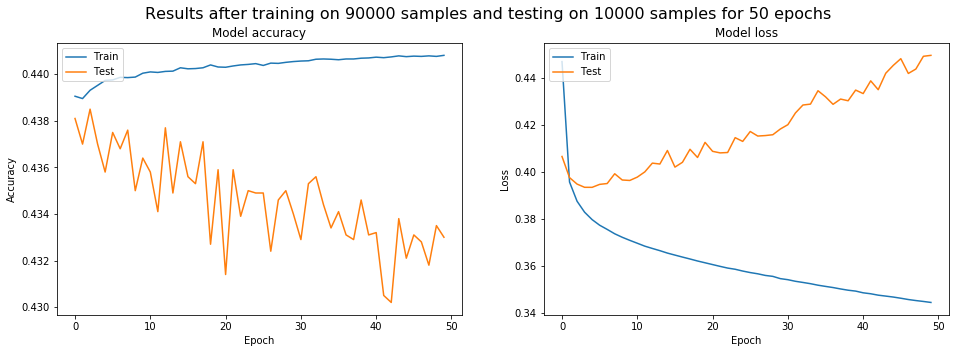
\includegraphics[width=\textwidth]{images/config1_100000samples_50epochs.png}
\caption{Risultati di \textit{accuracy} e \textit{loss} dopo un training della rete neurale in configurazione 1 con 90.000 esempi e testing con 10.000 esempi per 50 iterazioni.}
\end{figure}




\section{Conclusioni}

\printbibliography[title={Riferimenti}]

\end{document}